\documentclass[11pt]{article}

\usepackage[margin=1in]{geometry}
\usepackage{amsmath,amssymb}
\usepackage{booktabs}
\usepackage{xcolor}
\usepackage{tikz}
\usepackage{float}
\usepackage[font=small,labelfont=bf,width=0.92\textwidth]{caption}
\usepackage{pgfplots}
\pgfplotsset{compat=1.18}
\usetikzlibrary{calc,arrows,positioning,fit,backgrounds,decorations.pathreplacing,patterns}

\definecolor{cElem}{RGB}{40,80,140}
\definecolor{cTrg}{RGB}{190,40,40}
\definecolor{cCell}{RGB}{225,238,248}
\definecolor{cAcc}{RGB}{240,200,120}
\definecolor{cGrey}{RGB}{120,120,120}
\definecolor{cVec}{RGB}{110,55,150}

\newcommand{\stepbox}[1]{%
  \par\medskip\noindent\textbf{\color{cElem}#1}\par\nopagebreak\smallskip}

\title{Singular quadrature in \texttt{QuadElemList}\\[2pt]
       \large the self- and near-interaction algorithms, step by step}
\author{}
\date{}

\begin{document}
\maketitle
\vspace{-3.5em}

\section{Setting}

A \texttt{QuadElemList} holds high-order quadrilateral surface patches. Each patch carries an
$N\times N$ tensor grid of Gauss--Legendre nodes on the reference square $[0,1]^2$, and the
surface is the order-$N$ polynomial interpolant of those nodes,
\[
  \mathbf{X}(u,v) \;=\; \sum_{i,j} \mathbf{x}_{ij}\, L_i(u) L_j(v),
  \qquad (u,v)\in[0,1]^2 .
\]
A boundary-integral operator needs, for a target $\mathbf{y}$ and a patch $E$,
\[
  U(\mathbf{y}) \;=\; \int_E K(\mathbf{y},\mathbf{x})\,\sigma(\mathbf{x})\,\mathrm{d}S(\mathbf{x}),
\]
assembled as a matrix acting on the patch's nodal density values. When $\mathbf{y}$ is far from
$E$ a smooth tensor rule suffices. Two cases need special treatment, and each has its own
algorithm:

\begin{center}
\begin{minipage}{\textwidth}\centering
\begin{tabular}{@{}lll@{}}
\toprule
 & \textbf{self} & \textbf{near} \\
\midrule
target & \emph{on} $E$, at a node $(u_0,v_0)$ & \emph{off} $E$, at distance $d\ll$ patch size \\
integrand & singular, $K\sim 1/r$ & nearly singular, sharply peaked \\
scheme & Duffy edge-collapse & split-at-foot refinement \\
entry point & \texttt{SelfInterac} & \texttt{NearInterac} \\
\bottomrule
\end{tabular}
\captionof{table}{Everything else --- a target far from the patch relative to its size --- takes a plain tensor
Gauss--Legendre rule and is not discussed here.}
\end{minipage}
\end{center}

Both entry points map the runtime element order to a compile-time \texttt{order} and the runtime
tolerance to a runtime \texttt{digits}; both are independent and may be called in either order.

\vspace{1em}
\hrule
\section{Self interaction: the Duffy edge-collapse}

The target sits \emph{on} the patch, at node $(u_0,v_0)$, so $r=|\mathbf{X}(u,v)-\mathbf{X}(u_0,v_0)|$
vanishes there and $K\sim1/r$ is not integrable by any smooth rule. The Duffy transform removes
the singularity through the Jacobian rather than by refinement.

\stepbox{Step 1 --- split the panel at the target}

Join the target to the four corners. This gives four triangles, each with the target as one
vertex and one edge of the square opposite it.

\begin{center}
\begin{minipage}{\textwidth}\centering
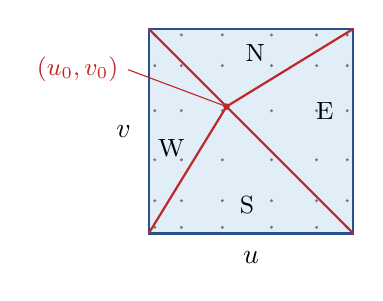
\begin{tikzpicture}[scale=2.6]
  \def\ux{0.38} \def\vy{0.62}
  \fill[cCell] (0,0) rectangle (1,1);
  \draw[cElem,thick] (0,0) rectangle (1,1);
  % GL-ish nodes
  \foreach \x in {0.03,0.16,0.36,0.60,0.82,0.97}
    \foreach \y in {0.03,0.16,0.36,0.60,0.82,0.97}
      \fill[cGrey] (\x,\y) circle (0.008);
  % the four triangles
  \draw[cTrg,thick] (\ux,\vy) -- (0,0);
  \draw[cTrg,thick] (\ux,\vy) -- (1,0);
  \draw[cTrg,thick] (\ux,\vy) -- (1,1);
  \draw[cTrg,thick] (\ux,\vy) -- (0,1);
  \fill[cTrg] (\ux,\vy) circle (0.016);
  \draw[cTrg,thin] (\ux,\vy) -- (-0.10,0.80);
  \node[cTrg,font=\small,left=0pt] at (-0.10,0.80) {$(u_0,v_0)$};
  \node[font=\small] at (0.48,0.14) {S};
  \node[font=\small] at (0.86,0.60) {E};
  \node[font=\small] at (0.52,0.88) {N};
  \node[font=\small] at (0.11,0.42) {W};
  \node[below] at (0.5,-0.04) {$u$};
  \node[left]  at (-0.04,0.5) {$v$};
\end{tikzpicture}
\captionof{figure}{Step 1. The target is always at a node, never at a corner or edge midpoint, so none of the four
triangles is degenerate.}
\end{minipage}
\end{center}

\stepbox{Step 2 --- collapse one edge onto the target}

Parametrise each triangle by $(s,t)\in[0,1]^2$ with
\[
  P(s,t) \;=\; (u_0,v_0) + s\,\mathbf{c}(t), \qquad \mathbf{c}(t) = (1-t)\,\mathbf{a} + t\,\mathbf{b},
\]
where $\mathbf{a}$ and $\mathbf{b}$ point from the target to the two ends of the opposite edge.
The line $s=0$ collapses the entire $t$-edge onto the target. The Jacobian is
\[
  \boxed{\;|\det| \;=\; s\,|\mathbf{a}\times\mathbf{b}|\;}
\]
--- linear in $s$, and \emph{independent of $t$}.

\begin{center}
\begin{minipage}{\textwidth}\centering
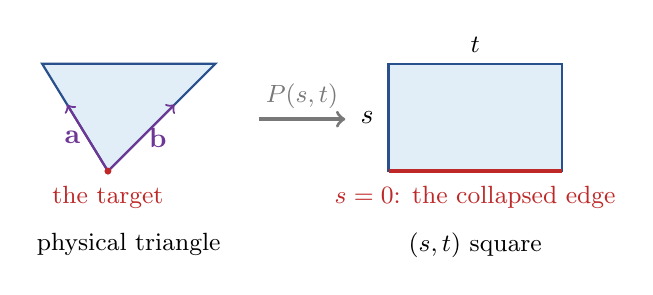
\begin{tikzpicture}[scale=2.2]
  % physical triangle
  \begin{scope}
    \fill[cCell] (0.38,0) -- (0,0.62) -- (1,0.62) -- cycle;
    \draw[cElem,thick] (0.38,0) -- (0,0.62) -- (1,0.62) -- cycle;
    \draw[->,cVec,thick] (0.38,0) -- ($(0.38,0)!0.62!(0,0.62)$) node[midway,left=-1pt] {$\mathbf{a}$};
    \draw[->,cVec,thick] (0.38,0) -- ($(0.38,0)!0.62!(1,0.62)$) node[midway,right=-1pt] {$\mathbf{b}$};
    \fill[cTrg] (0.38,0) circle (0.02);
    \node[cTrg,below,font=\small] at (0.38,-0.03) {the target};
    \node[below,font=\small] at (0.5,-0.30) {physical triangle};
  \end{scope}
  % arrow
  \draw[->,very thick,cGrey] (1.25,0.3) -- (1.75,0.3) node[midway,above] {\small $P(s,t)$};
  % (s,t) square
  \begin{scope}[xshift=2cm]
    \fill[cCell] (0,0) rectangle (1,0.62);
    \draw[cElem,thick] (0,0) rectangle (1,0.62);
    \draw[cTrg,ultra thick] (0,0) -- (1,0);
    \node[cTrg,below,font=\small] at (0.5,-0.03) {$s=0$: the collapsed edge};
    \node[left] at (-0.03,0.31) {$s$};
    \node[below,font=\small] at (0.5,-0.30) {$(s,t)$ square};
    \node[above,font=\small] at (0.5,0.63) {$t$};
  \end{scope}
\end{tikzpicture}
\captionof{figure}{Step 2. The entire edge $s=0$ maps to the single target point.}
\end{minipage}
\end{center}

That single factor of $s$ is the whole point. For a kernel of order $1/r$, writing
$\|\cdot\|_G$ for the length induced by the surface metric $G$ at the target,
\[
  K\,|\det| \;\sim\; \frac{1}{s\,\|\mathbf{c}(t)\|_G}\cdot s\,|\mathbf{a}\times\mathbf{b}|
             \;=\; \frac{|\mathbf{a}\times\mathbf{b}|}{\|\mathbf{c}(t)\|_G},
\]
which is bounded as $s\to0$. The singularity is gone.

\stepbox{Step 3 --- pick the two rules}

The $s$-direction is now smooth, so it takes a plain Gauss--Legendre rule with $q_s=N$ nodes.
The $t$-direction keeps a residual peak: $1/\|\mathbf{c}(t)\|_G$ is largest where $\mathbf{c}(t)$
is shortest, at the foot $t^\ast$ of the perpendicular from the target to the far edge. The peak
has height $\sim 1/d$ and width $\sim d/L$, where $d$ is the distance to that edge and $L$ its
length.

Both $t^\ast$ and $d/L$ are computed in the \emph{surface} metric $G$, not in parameter space:
using parameter distances misplaces the peak by $|\cot\theta|$ peak-widths on a sheared patch.
The peak is then resolved by a $\sinh$ substitution,
\[
  t \;=\; t^\ast + \tfrac{d}{L}\sinh\xi ,
\]
with one GL rule of $n_t$ points in $\xi$. $n_t$ grows with the requested digits and is larger
for vector kernels than scalar ones.

\begin{center}
\begin{minipage}{\textwidth}\centering
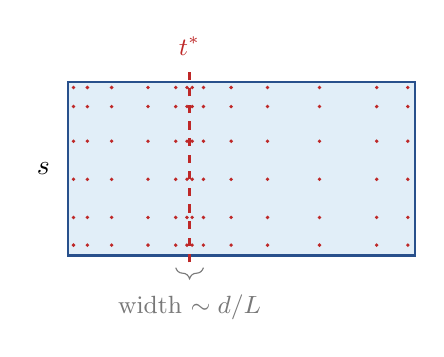
\begin{tikzpicture}[scale=2.2]
  \fill[cCell] (0,0) rectangle (2,1);
  \draw[cElem,thick] (0,0) rectangle (2,1);
  \node[left] at (-0.05,0.5) {$s$};
  \foreach \s in {0.06,0.22,0.44,0.66,0.86,0.97} {
    \foreach \t in {0.03,0.11,0.25,0.46,0.62,0.685,0.715,0.78,0.94,1.15,1.45,1.78,1.96} {
      \fill[cTrg] (\t,\s) circle (0.011);
    }
  }
  \draw[dashed,cTrg,thick] (0.70,-0.04) -- (0.70,1.10);
  \node[cTrg,above,font=\small] at (0.70,1.10) {$t^\ast$};
  \draw[decorate,decoration={brace,amplitude=4pt,mirror},cGrey] (0.62,-0.07) -- (0.78,-0.07);
  \node[cGrey,below,font=\small] at (0.70,-0.17) {width $\sim d/L$};
\end{tikzpicture}
\captionof{figure}{Step 3. One triangle of the four, $n_s\times n_t$ points each.}
\end{minipage}
\end{center}

\stepbox{Step 4 --- contract, evaluate, project}

Everything above depends only on $(N,t_i,t_j,\text{triangle})$, so the interpolation operators are
built once per order and cached. The collapse gives them structure: for the S triangle
$v(s,t)=v_0(1-s)$ depends on $s$ alone, so that factor is a small $(N\times n_s)$ operator rather
than $(N \times n_s n_t)$. The evaluation is then a chain of GEMMs:

\begin{center}
\begin{minipage}{\textwidth}\centering
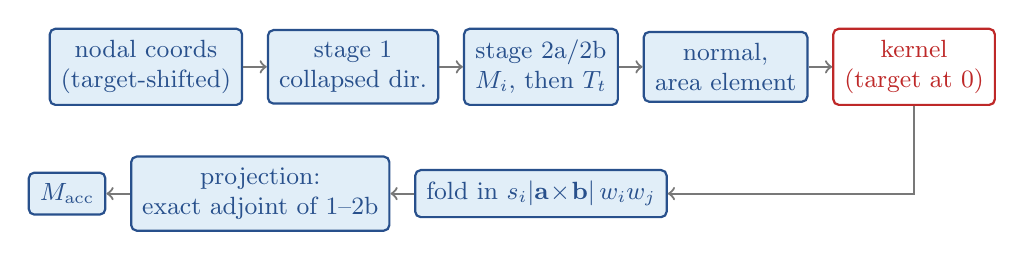
\begin{tikzpicture}[node distance=3mm,
   b/.style={draw,cElem,thick,fill=cCell,rounded corners=2pt,align=center,inner sep=4pt,font=\small},
   k/.style={draw,cTrg,thick,fill=white,rounded corners=2pt,align=center,inner sep=4pt,font=\small},
   a/.style={->,thick,cGrey}]
  \node[b] (f)  {nodal coords\\ (target-shifted)};
  \node[b,right=of f]  (s1) {stage 1\\ collapsed dir.};
  \node[b,right=of s1] (s2) {stage 2a/2b\\ $M_i$, then $T_t$};
  \node[b,right=of s2] (g)  {normal,\\ area element};
  \node[k,right=of g]  (kk) {kernel\\ (target at $0$)};
  \draw[a] (f)--(s1); \draw[a] (s1)--(s2); \draw[a] (s2)--(g); \draw[a] (g)--(kk);
  \node[b,below=8mm of s2] (w) {fold in $s_i|\mathbf{a}\!\times\!\mathbf{b}|\,w_i w_j$};
  \node[b,left=of w] (p) {projection:\\ exact adjoint of 1--2b};
  \node[b,left=of p] (m) {$M_{\text{acc}}$};
  \draw[a] (kk) |- (w); \draw[a] (w)--(p); \draw[a] (p)--(m);
\end{tikzpicture}
\captionof{figure}{Step 4. One target, one triangle. Blue boxes are GEMMs against operators cached per
$(N,\text{digits})$; the kernel sees the target at the origin because the nodal coordinates are
stored target-shifted.}
\end{minipage}
\end{center}

The projection reuses the same operators in reverse order, so it is the exact adjoint of the
interpolation --- which is what keeps the assembled operator consistent. Sources are stored
relative to the target, so the kernel is always evaluated with the target at the origin and $r$
stays accurate near the singularity.

\vspace{1em}
\hrule
\section{Near interaction: split at the foot}

Here the target is \emph{off} the patch at a distance $d$ that may be far smaller than the patch.
The integrand is smooth but sharply peaked near the closest point, and a single tensor rule would
need impractically many points. The scheme refines --- but chooses \emph{where} to refine so that
every operator can be precomputed.

\stepbox{Step 1 --- find the foot}

Locate $(u^\ast,v^\ast)$ minimising $|\mathbf{X}(u,v)-\mathbf{y}|^2$ over $[0,1]^2$: seed at the
nearest nodal point, then Gauss--Newton on the first fundamental form, clamped to the box with a
backtracking line search, falling back to a shrinking grid search if it stalls. Optimality is
tested on the \emph{projected} gradient, since at a box edge the constrained gradient is large --
it balances the constraint -- and near-pair feet usually do lie on a shared patch edge.

\begin{center}
\begin{minipage}{\textwidth}\centering
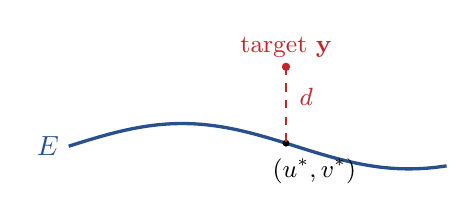
\begin{tikzpicture}[scale=2.4]
  \draw[cElem,very thick] plot[smooth,domain=0:2,samples=40] (\x,{0.12*sin(150*\x)});
  \node[cElem,left] at (0,0) {$E$};
  \fill[cTrg] (1.15,0.42) circle (0.022) node[above,cTrg,font=\small] {target $\mathbf{y}$};
  \fill[black] (1.15,{0.12*sin(150*1.15)}) circle (0.018);
  \node[below,font=\small] at (1.30,{0.12*sin(150*1.15)-0.03}) {$(u^\ast,v^\ast)$};
  \draw[dashed,cTrg] (1.15,0.42) -- (1.15,{0.12*sin(150*1.15)});
  \node[cTrg,right,font=\small] at (1.17,0.26) {$d$};
\end{tikzpicture}
\captionof{figure}{Near, step 1. The foot is found by Gauss--Newton from the nearest nodal point. $d$ may be far
smaller than the patch, which is what makes the integrand nearly singular.}
\end{minipage}
\end{center}

\stepbox{Step 2 --- split the patch \emph{at} the foot}

Cut the parameter square along $u=u^\ast$ and $v=v^\ast$, giving four sub-elements. Every
sub-element now has the foot at one \emph{corner}, so refinement always grades toward an
\emph{endpoint} of the sub-element rather than to a point in its interior.

\begin{center}
\begin{minipage}{\textwidth}\centering
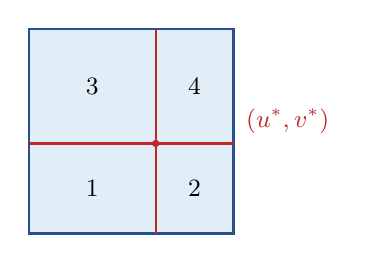
\begin{tikzpicture}[scale=2.6]
  \def\ux{0.62} \def\vy{0.44}
  \fill[cCell] (0,0) rectangle (1,1);
  \draw[cElem,thick] (0,0) rectangle (1,1);
  \draw[cTrg,thick] (\ux,0) -- (\ux,1);
  \draw[cTrg,thick] (0,\vy) -- (1,\vy);
  \fill[cTrg] (\ux,\vy) circle (0.018);
  \node[cTrg,font=\small,above right=0pt and 1pt] at (1.0,\vy) {$(u^\ast,v^\ast)$};
  \node[font=\small] at (0.31,0.22) {1};
  \node[font=\small] at (0.81,0.22) {2};
  \node[font=\small] at (0.31,0.72) {3};
  \node[font=\small] at (0.81,0.72) {4};
\end{tikzpicture}
\captionof{figure}{Near, step 2. With the foot at a corner of every sub-element, refinement grades toward an
endpoint and the graded intervals depend only on the level --- which is what lets the operators
be tabulated per $N$ rather than rebuilt per target.}
\end{minipage}
\end{center}

This is the step that makes the scheme cheap. In \emph{normalised} sub-element coordinates the
graded intervals depend only on the refinement level, never on $(u^\ast,v^\ast)$, so their
interpolation operators are built once per order and looked up. A bisection quadtree, by
contrast, leaves the foot mid-cell and needs a position-dependent operator per leaf --- hundreds
of small matrices rebuilt for every target.

\stepbox{Step 3 --- bisect until admissible}

Within a sub-element, normalise so the foot is at $x=1$. The graded intervals are
\[
  \text{shell}_k = [\,1-2^{-k},\; 1-2^{-(k+1)}\,], \qquad
  \text{core}_k  = [\,1-2^{-k},\; 1\,],
\]
i.e.\ $\text{core}_k$ is the part still touching the foot and $\text{shell}_k$ the half turned away
from it.

Splitting at the foot leaves the sub-elements \emph{anisotropic}, so quadrisection would hand that
aspect ratio down to every descendant. Instead the corner cell is bisected along its longer
\emph{physical} dimension only --- parameter extent times surface speed --- one split at a time,
until that dimension is admissible against the target distance:
\[
  b_{\text{ellipse}}\cdot\max(h_u,h_v) \;\le\; d .
\]
Each split emits exactly one leaf (the half not touching the corner), and the $u$- and
$v$-levels advance independently.

\begin{center}
\begin{minipage}{\textwidth}\centering
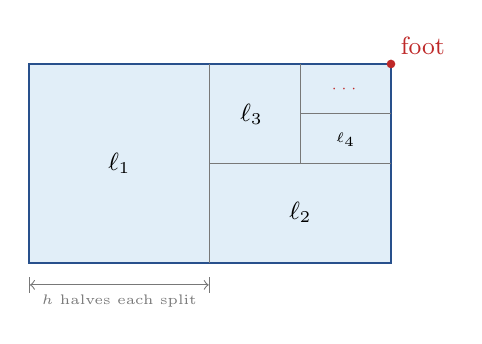
\begin{tikzpicture}[scale=4.6,font=\small]
  \fill[cCell] (0,0) rectangle (1,0.55);
  \draw[cElem,thick] (0,0) rectangle (1,0.55);
  % bisections marching toward the foot at (1,0.55)
  \draw[cGrey] (0.5,0) -- (0.5,0.55);
  \draw[cGrey] (0.5,0.275) -- (1,0.275);
  \draw[cGrey] (0.75,0.275) -- (0.75,0.55);
  \draw[cGrey] (0.75,0.4125) -- (1,0.4125);
  \fill[cTrg] (1,0.55) circle (0.012);
  \node[cTrg,above right=0pt,font=\small] at (1,0.55) {foot};
  \node at (0.25,0.275) {$\ell_1$};
  \node at (0.75,0.14)  {$\ell_2$};
  \node at (0.615,0.41) {$\ell_3$};
  \node at (0.875,0.34) {\tiny $\ell_4$};
  \node[cTrg,font=\tiny] at (0.875,0.48) {$\cdots$};
  \draw[|<->|,cGrey] (0,-0.06) -- (0.5,-0.06) node[midway,below,font=\tiny] {$h$ halves each split};
\end{tikzpicture}
\captionof{figure}{Near, step 3. The corner cell is split along its longer \emph{physical} dimension (parameter
extent $\times$ surface speed) until $b_{\text{ellipse}}\max(h_u,h_v)\le d$, one leaf per split,
the $u$- and $v$-levels advancing independently. Roughly ten leaves per target at the tolerances
used here.}
\end{minipage}
\end{center}

\stepbox{Step 4 --- choose the per-cell order}

Each leaf gets a Gauss--Legendre rule whose order comes from the tolerance, via a Bernstein-ellipse
argument evaluated at the \emph{end-foot} reach (the foot lands on a cell endpoint, which is a
weaker requirement than the semi-major reach by $a^2/b^2\approx1.9$).

That test lives in parameter space and cannot see one thing: how skewed the patch is where the
target sits. The required order is flat up to a corner angle of about $120^\circ$ and then grows
like $1/(180^\circ-\varphi)$ as the corner flattens and the element wraps around the target. So
the order is corrected per (element, target) using $\varphi$, the acute angle between the surface
tangents \emph{at the foot}. An orthogonal parametrisation gives $\varphi=90^\circ$, a correction
factor of $1$, and costs a well-shaped mesh nothing.

\begin{center}
\begin{minipage}{\textwidth}\centering
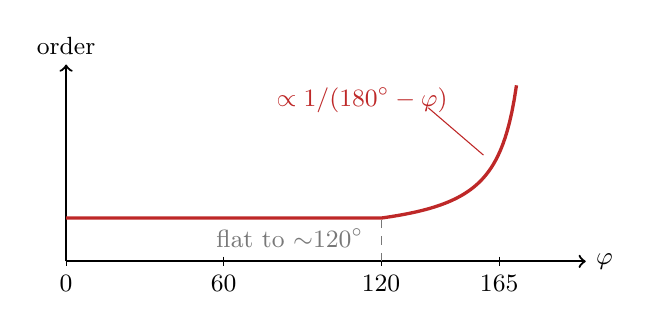
\begin{tikzpicture}[scale=1.0]
  \draw[->,thick] (0,0) -- (6.6,0) node[right,font=\small] {$\varphi$};
  \draw[->,thick] (0,0) -- (0,2.5) node[above,font=\small] {order};
  \foreach \x/\l in {0/0,2/60,4/120,5.5/165} \draw (\x,0.06)--(\x,-0.06) node[below,font=\small] {\l};
  \draw[cTrg,very thick] (0,0.55) -- (4,0.55)
        plot[domain=4:5.72,samples=60] (\x,{0.55+0.55/(6.0-\x)-0.55/2.0});
  \node[cTrg,font=\small,anchor=west] at (2.55,2.05) {$\propto 1/(180^\circ-\varphi)$};
  \draw[cTrg,thin] (4.6,1.95) -- (5.3,1.35);
  \draw[dashed,cGrey] (4,0)--(4,0.55);
  \node[cGrey,font=\small,anchor=east] at (3.9,0.30) {flat to $\sim$120$^\circ$};
\end{tikzpicture}
\captionof{figure}{Near, step 4. Schematic, not measured. $\varphi$ is the acute angle between the surface tangents
at the foot; an orthogonal parametrisation sits at $\varphi=90^\circ$ and needs no correction.}
\end{minipage}
\end{center}

\stepbox{Step 5 --- integrate each leaf and accumulate}

Each sub-element's nodal coordinates are built once per target
($X_{\text{sub}} = S_u^{\!\top}\,\mathbf{x}\,S_v$), so nothing depending on $(u^\ast,v^\ast)$
survives into the per-cell loop. Every leaf then runs the same tensor-product block:

\begin{center}
\begin{minipage}{\textwidth}\centering
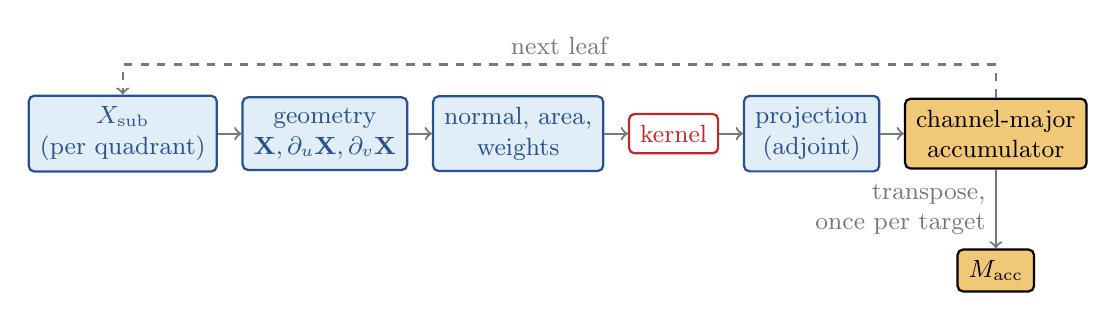
\begin{tikzpicture}[node distance=3mm,
   b/.style={draw,cElem,thick,fill=cCell,rounded corners=2pt,align=center,inner sep=4pt,font=\small},
   k/.style={draw,cTrg,thick,fill=white,rounded corners=2pt,align=center,inner sep=4pt,font=\small},
   o/.style={draw,thick,fill=cAcc,rounded corners=2pt,align=center,inner sep=4pt,font=\small},
   a/.style={->,thick,cGrey}]
  \node[b] (x)  {$X_{\text{sub}}$\\ (per quadrant)};
  \node[b,right=of x]  (gt) {geometry\\ $\mathbf{X},\partial_u\mathbf{X},\partial_v\mathbf{X}$};
  \node[b,right=of gt] (as) {normal, area,\\ weights};
  \node[k,right=of as] (kk) {kernel};
  \node[b,right=of kk] (pr) {projection\\ (adjoint)};
  \node[o,right=of pr] (ac) {channel-major\\ accumulator};
  \draw[a] (x)--(gt); \draw[a] (gt)--(as); \draw[a] (as)--(kk); \draw[a] (kk)--(pr); \draw[a] (pr)--(ac);
  \node[o,below=10mm of ac] (mm) {$M_{\text{acc}}$};
  \draw[a] (ac)--(mm) node[midway,left,align=right,font=\small] {transpose,\\once per target};
  \draw[a,dashed] (ac.north) -- ++(0,0.42) -| (x.north)
        node[pos=0.25,above,font=\small] {next leaf};
\end{tikzpicture}
\captionof{figure}{Near, step 5. $X_{\text{sub}}$ is built once per target, so nothing depending on
$(u^\ast,v^\ast)$ enters the loop. The channel-major accumulator lets the projection's final
GEMM add in place ($\beta=1$).}
\end{minipage}
\end{center}

Cells accumulate into a channel-major buffer so the projection's last GEMM can add in place
($\beta=1$); a single transpose into the node-major layout at the end replaces a per-cell sweep.

\vspace{1em}
\hrule
\section{Numerical results}

All from \texttt{bench-cubed-sphere}. The surface is a cubed sphere twisted about $z$.

\begin{figure}[H]\centering
\input{fig-cubed-sphere}
\caption{$4\times4$ patches per face; the runs below use $8\times8$ and $12\times12$. The twist is an
\emph{isometry}, so all four panels are the same unit sphere and only the parametrisation shears
--- every difference in the tables below is therefore caused by the parametrisation alone. At
$\theta=\pi$ the patch edges are far from orthogonal, which is where the corner angle $\varphi$
of Section~3, Step~4 departs from $90^\circ$.}
\end{figure}

\subsection{Convergence}

Order 12, 12 patches per face ($864$ elements, $124{,}416$ nodes). \emph{error} is the on-surface
Green's identity $S[\partial_n u]-D[u]=u$, relative to $\max|u|$; \emph{error-density} is the
interpolation error of the two densities at off-node parameters, i.e.\ how well the order-12
patch represents them. The last three columns give the cost of that accuracy on each of the three machines.

\begin{table}[H]\centering\small
\begin{tabular}{@{}llllrrr@{}}
\toprule
 & & & & \multicolumn{3}{c}{pts/s/core, SL setup} \\
\cmidrule(l){5-7}
kernel, twist & tol & error-density & error & Rome & Genoa & Icelake \\
\midrule

laplace, $\pi/6$ & $1.00\!\times\!10^{-3}$ & $7.18\!\times\!10^{-14}$ & $2.14\!\times\!10^{-7}$ & 3628 & 8547 & 6677 \\
 & $1.00\!\times\!10^{-6}$ & $7.18\!\times\!10^{-14}$ & $3.73\!\times\!10^{-10}$ & 3162 & 6861 & 6242 \\
 & $1.00\!\times\!10^{-9}$ & $7.18\!\times\!10^{-14}$ & $3.42\!\times\!10^{-12}$ & 2444 & 4972 & 4958 \\
 & $1.00\!\times\!10^{-12}$ & $7.18\!\times\!10^{-14}$ & $3.32\!\times\!10^{-13}$ & 1631 & 3247 & 3591 \\
\addlinespace
laplace, $\pi/2$ & $1.00\!\times\!10^{-3}$ & $4.89\!\times\!10^{-11}$ & $2.44\!\times\!10^{-7}$ & 3326 & 7287 & 7739 \\
 & $1.00\!\times\!10^{-6}$ & $4.89\!\times\!10^{-11}$ & $8.52\!\times\!10^{-10}$ & 2405 & 4822 & 4808 \\
 & $1.00\!\times\!10^{-9}$ & $4.89\!\times\!10^{-11}$ & $4.07\!\times\!10^{-11}$ & 1668 & 3221 & 3271 \\
 & $1.00\!\times\!10^{-12}$ & $4.89\!\times\!10^{-11}$ & $2.71\!\times\!10^{-12}$ & 1066 & 2104 & 2149 \\
\addlinespace
laplace, $\pi$ & $1.00\!\times\!10^{-3}$ & $4.28\!\times\!10^{-8}$ & $2.02\!\times\!10^{-6}$ & 1944 & 3822 & 3867 \\
 & $1.00\!\times\!10^{-6}$ & $4.28\!\times\!10^{-8}$ & $1.63\!\times\!10^{-8}$ & 943 & 1839 & 1701 \\
 & $1.00\!\times\!10^{-9}$ & $4.28\!\times\!10^{-8}$ & $2.04\!\times\!10^{-10}$ & 539 & 1031 & 952 \\
 & $1.00\!\times\!10^{-12}$ & $4.28\!\times\!10^{-8}$ & $4.65\!\times\!10^{-11}$ & 316 & 606 & 551 \\
\addlinespace
stokes, $\pi/6$ & $1.00\!\times\!10^{-3}$ & $2.25\!\times\!10^{-13}$ & $4.25\!\times\!10^{-6}$ & 2277 & 5024 & 4681 \\
 & $1.00\!\times\!10^{-6}$ & $2.25\!\times\!10^{-13}$ & $4.66\!\times\!10^{-9}$ & 1696 & 3650 & 3062 \\
 & $1.00\!\times\!10^{-9}$ & $2.25\!\times\!10^{-13}$ & $1.07\!\times\!10^{-10}$ & 1204 & 2605 & 2149 \\
 & $1.00\!\times\!10^{-12}$ & $2.25\!\times\!10^{-13}$ & $7.68\!\times\!10^{-12}$ & 815 & 1708 & 1546 \\
\addlinespace
stokes, $\pi/2$ & $1.00\!\times\!10^{-3}$ & $1.54\!\times\!10^{-10}$ & $8.06\!\times\!10^{-6}$ & 1946 & 4108 & 3691 \\
 & $1.00\!\times\!10^{-6}$ & $1.54\!\times\!10^{-10}$ & $3.10\!\times\!10^{-8}$ & 1219 & 2139 & 2199 \\
 & $1.00\!\times\!10^{-9}$ & $1.54\!\times\!10^{-10}$ & $8.89\!\times\!10^{-10}$ & 800 & 1693 & 1443 \\
 & $1.00\!\times\!10^{-12}$ & $1.54\!\times\!10^{-10}$ & $5.98\!\times\!10^{-11}$ & 521 & 1093 & 874 \\
\addlinespace
stokes, $\pi$ & $1.00\!\times\!10^{-3}$ & $1.58\!\times\!10^{-7}$ & $1.36\!\times\!10^{-5}$ & 1010 & 2099 & 1843 \\
 & $1.00\!\times\!10^{-6}$ & $1.58\!\times\!10^{-7}$ & $1.10\!\times\!10^{-7}$ & 420 & 902 & 782 \\
 & $1.00\!\times\!10^{-9}$ & $1.58\!\times\!10^{-7}$ & $8.76\!\times\!10^{-10}$ & 235 & 496 & 430 \\
 & $1.00\!\times\!10^{-12}$ & $1.58\!\times\!10^{-7}$ & $3.19\!\times\!10^{-10}$ & 137 & 286 & 250 \\
\bottomrule
\end{tabular}
\caption{Order 12, 12 patches per face ($864$ elements, $124{,}416$ nodes), single point source outside
the surface. \emph{error} is $\max|(S[\partial_n
u]-D[u])-u|/\max|u|$ at the surface nodes, so it exercises both operators together. The two
error columns are from Rome; Genoa and Icelake agree to the digits shown. Throughput is the
single-layer setup with each machine on all of its cores, so it carries that machine's parallel
efficiency.}
\end{table}

\begin{itemize}\setlength\itemsep{1pt}
\item \textbf{The geometry is never the limit} --- it resolves to $\sim10^{-15}$ at every twist
      (not shown).
\item \textbf{The error tracks the tolerance over nine decades}: at twist $\pi/6$,
      $2.1\times10^{-7}\!\to\!3.3\times10^{-13}$.
\item \textbf{It stops at a floor set by the parametrisation}, and that floor degrades sharply
      with twist --- at $\pi$ the best Laplace result is $4.7\times10^{-11}$ against
      $3.3\times10^{-13}$ at $\pi/6$, a factor of $140$ for the same mesh and tolerance.
\item \textbf{\emph{error-density} is a resolution indicator, not a bound}: at high twist the
      error sits well below it ($4.7\times10^{-11}$ versus $4.3\times10^{-8}$), because the
      identity is tested at nodes, where the densities are exact, and the quadrature averages the
      between-node error.
\end{itemize}

\noindent
The throughput columns say where the cost goes, and it is not where the tolerance is.

\begin{itemize}\setlength\itemsep{1pt}
\item \textbf{Tolerance is cheap} --- nine decades cost about a factor of two (Laplace, $\pi/6$,
      Rome: $3628$ pts/s/core at $10^{-3}$, still $1631$ at $10^{-12}$).
\item \textbf{Twist is expensive} --- at a fixed tolerance of $10^{-9}$ Laplace falls from $2444$ to
      $539$ pts/s/core between $\pi/6$ and $\pi$, a factor of $4.5$ on Rome and $4.8$--$5.2$ on
      Genoa and Icelake.
\item \textbf{So a sheared parametrisation is penalised twice}, once in accuracy and again in
      time, for the same mesh and the same requested tolerance. Both are the near scheme reacting
      to the corner angle $\varphi$: a skewed patch raises the per-cell order and deepens the
      refinement, for every target.
\item \textbf{The machine ratio, by contrast, barely moves} --- median $1.98$ over all $48$
      machine-to-Rome comparisons, every one between $1.68$ and $2.36$. The architecture gap sits
      in the kernel evaluation, not in how hard the quadrature is working.
\end{itemize}

\subsection{OpenMP scaling}

Order 12, 8 patches per face ($384$ elements, $55{,}296$ nodes), twist $\pi/6$, tol $10^{-9}$;
self- and near-interaction setup, with
\texttt{OMP\_PLACES=cores} and \texttt{OMP\_PROC\_BIND=close}. Everything below is the \emph{single-layer} operator alone --- the driver times the two setups
separately, and the double-layer setup, which takes essentially the same time again, is not included. Three node types:

\begin{table}[H]\centering\small
\begin{tabular}{@{}llll@{}}
\toprule
 & cores & AVX-512 & build \\
\midrule
AMD EPYC 7742 (Rome)      & $2\times64$ & no  & \texttt{-march=native} $\to$ AVX2 \\
AMD EPYC 9474F (Genoa)    & $2\times48$ & yes & \texttt{-march=native} $\to$ AVX-512 \\
Intel Xeon 8358 (Icelake) & $2\times32$ & yes & \texttt{-march=native} $\to$ AVX-512 \\
\bottomrule
\end{tabular}
\caption{Run \texttt{-{}-exclusive}, one MPI rank per node.}
\end{table}

\begin{table}[H]\centering\small
\begin{tabular}{@{}llrrrrrr@{}}
\toprule
 & & & \multicolumn{2}{c}{1 thread} & \multicolumn{2}{c}{full node} & \\
\cmidrule(lr){4-5}\cmidrule(lr){6-7}
machine & kernel & cores & setup (s) & pts/s & setup (s) & pts/s & speedup \\
\midrule
Rome    & Laplace & 128 & 15.382 & 3595 & 0.183 & 301\,645 & 84.1$\times$ (66\%) \\
Genoa   & Laplace &  96 &  9.546 & 5793 & 0.121 & 457\,565 & 78.9$\times$ (82\%) \\
Icelake & Laplace &  64 &  8.764 & 6310 & 0.177 & 313\,018 & 49.5$\times$ (77\%) \\
\addlinespace
Rome    & Stokes  & 128 & 30.347 & 1822 & 0.387 & 142\,835 & 78.4$\times$ (61\%) \\
Genoa   & Stokes  &  96 & 18.117 & 3052 & 0.223 & 248\,323 & 81.2$\times$ (85\%) \\
Icelake & Stokes  &  64 & 18.977 & 2914 & 0.410 & 134\,861 & 46.3$\times$ (72\%) \\
\bottomrule
\end{tabular}
\caption{\emph{setup} is the total wall time of the self- and near-interaction setup, single layer only,
at order 12, 8 patches per face ($384$ elements, $N=55{,}296$ nodes), twist $\pi/6$, tol
$10^{-9}$. The double-layer setup costs the same to within a few percent at every thread count on all three
machines, so building both operators takes about twice the times listed.}
\end{table}

\begin{itemize}\setlength\itemsep{1pt}
\item \textbf{Per core at one thread}, Icelake and Genoa are $1.6$--$1.8\times$ Rome (Laplace
      $6310$ and $5793$ against $3595$). Rome is the only one of the three without AVX-512 and the
      only one compiled to AVX2, so that is the expected place for the vector width to show.
\item \textbf{All three lose per-core throughput as threads are added}, Rome most: $-34\%$ from 1
      thread to 128, against $-18\%$ (Genoa, to 96) and $-22\%$ (Icelake, to 64).
\item \textbf{Genoa holds $82$--$85\%$ efficiency at 96 threads} where Rome is at $61$--$66\%$ at
      128. Part of that is Rome being asked to go further, but Rome is also below Genoa at the
      same thread count ($72\%$ against $89\%$ at 64 threads, Laplace).
\item \textbf{On absolute throughput the core counts stop cancelling}: Genoa is highest despite
      having a third fewer cores than Rome, and Icelake matches Rome with half of them.
\item \textbf{The self loop runs short of work at the widest counts}: only $384/N$ elements per
      thread, 3 per thread on Rome at 128, which is coarse for \texttt{schedule(static)}. That
      is what bounds every curve at the right-hand end.
\item \textbf{Stokes sits uniformly a little below Laplace}, consistent with its larger per-target
      working set.
\end{itemize}

\begin{figure}[H]\centering
\begin{tikzpicture}
\begin{axis}[width=0.49\textwidth,height=4.9cm,xmode=log,ymode=log,log basis x=2,log basis y=2,
             xlabel={threads},ylabel={speedup},xmin=0.8,xmax=160,ymin=0.8,ymax=160,
             legend pos=north west,legend style={font=\scriptsize,draw=none},
             grid=both,grid style={cGrey!20},tick label style={font=\scriptsize},
             label style={font=\small},title style={font=\small},title={Laplace}]
  \addplot[dashed,cGrey,thick,domain=1:128,samples=2]{x}; \addlegendentry{ideal}
  \addplot[cElem,thick,mark=*,mark size=1.4] table[x=thr,y=speedup] {data/scaling-rome-laplace.dat};
  \addlegendentry{Rome}
  \addplot[cTrg,thick,mark=square*,mark size=1.4] table[x=thr,y=speedup] {data/scaling-genoa-laplace.dat};
  \addlegendentry{Genoa}
  \addplot[black,thick,mark=triangle*,mark size=1.8] table[x=thr,y=speedup] {data/scaling-icelake-laplace.dat};
  \addlegendentry{Icelake}
\end{axis}
\end{tikzpicture}
\hfill
\begin{tikzpicture}
\begin{axis}[width=0.49\textwidth,height=4.9cm,xmode=log,log basis x=2,
             xlabel={threads},ylabel={points/s/core},xmin=0.8,xmax=160,ymin=0,ymax=7000,
             legend pos=south west,legend style={font=\scriptsize,draw=none},
             grid=both,grid style={cGrey!20},tick label style={font=\scriptsize},
             label style={font=\small},title style={font=\small},title={Laplace}]
  \addplot[cElem,thick,mark=*,mark size=1.4] table[x=thr,y=pps] {data/scaling-rome-laplace.dat};
  \addlegendentry{Rome}
  \addplot[cTrg,thick,mark=square*,mark size=1.4] table[x=thr,y=pps] {data/scaling-genoa-laplace.dat};
  \addlegendentry{Genoa}
  \addplot[black,thick,mark=triangle*,mark size=1.8] table[x=thr,y=pps] {data/scaling-icelake-laplace.dat};
  \addlegendentry{Icelake}
\end{axis}
\end{tikzpicture}

\vspace{4pt}

\begin{tikzpicture}
\begin{axis}[width=0.49\textwidth,height=4.9cm,xmode=log,log basis x=2,
             xlabel={threads},ylabel={parallel efficiency (\%)},xmin=0.8,xmax=160,ymin=0,ymax=105,
             legend pos=south west,legend style={font=\scriptsize,draw=none},
             grid=both,grid style={cGrey!20},tick label style={font=\scriptsize},
             label style={font=\small},title style={font=\small},title={Laplace}]
  \addplot[dashed,cGrey,thick,domain=1:128,samples=2,forget plot]{100};
  \addplot[cElem,thick,mark=*,mark size=1.4] table[x=thr,y=eff] {data/scaling-rome-laplace.dat};
  \addlegendentry{Rome}
  \addplot[cTrg,thick,mark=square*,mark size=1.4] table[x=thr,y=eff] {data/scaling-genoa-laplace.dat};
  \addlegendentry{Genoa}
  \addplot[black,thick,mark=triangle*,mark size=1.8] table[x=thr,y=eff] {data/scaling-icelake-laplace.dat};
  \addlegendentry{Icelake}
\end{axis}
\end{tikzpicture}
\hfill
\begin{tikzpicture}
\begin{axis}[width=0.49\textwidth,height=4.9cm,xmode=log,log basis x=2,
             xlabel={threads},ylabel={points/s/core},xmin=0.8,xmax=160,ymin=0,ymax=3500,
             legend pos=south west,legend style={font=\scriptsize,draw=none},
             grid=both,grid style={cGrey!20},tick label style={font=\scriptsize},
             label style={font=\small},title style={font=\small},title={Stokes}]
  \addplot[cElem,thick,mark=*,mark size=1.4] table[x=thr,y=pps] {data/scaling-rome-stokes.dat};
  \addlegendentry{Rome}
  \addplot[cTrg,thick,mark=square*,mark size=1.4] table[x=thr,y=pps] {data/scaling-genoa-stokes.dat};
  \addlegendentry{Genoa}
  \addplot[black,thick,mark=triangle*,mark size=1.8] table[x=thr,y=pps] {data/scaling-icelake-stokes.dat};
  \addlegendentry{Icelake}
\end{axis}
\end{tikzpicture}
\caption{Single-layer setup at order 12, 8 patches per face ($384$ elements, $N=55{,}296$ nodes), twist
$\pi/6$, tol $10^{-9}$. The double layer is timed separately and is not folded in; it costs about the same again. Speedup and
efficiency are against 1 thread on the same machine.}
\end{figure}

\end{document}
